\section{The line-of-sight floor}
\label{sec:lambdamin}

\subsection{What is cut, and why it depends on source redshift}

The vertex table's shells begin at $\lambda = 396.63$ Mpc and the callable
returns exactly zero outside them, so everything nearer than that
contributes nothing to the fold. Because $\lambda$ is measured from the
observer, that floor always corresponds to $z = 0.100$, whatever the source
redshift: what is excised is always the $z<0.1$ foreground.

The production fold uses a 24-node Gauss-Legendre rule whose nodes span
$[5.6, 2307.5]$ Mpc, six of which fall below the floor. By plain measure
that is $15\%$ of the integration range, but plain measure is the wrong
weight: the lensing efficiency $K = a^2\chi(\chi_s-\chi)/\chi_s$ vanishes
toward the observer, and the FK term carries four response lines, so $K^2$
and $K^4$ bracket the weighting. Both fractions grow as the source moves
nearer, which is the reason this matters for the multi-redshift figure and
not for the main analysis.

\begin{table}[h]
\centering
\begin{tabular}{rrrrr}
\toprule
$z_s$ & $\lambda_s$ [Mpc] & path fraction & $K^2$ weight & $K^4$ weight \\
\midrule
5.0 & 2318.0 & 0.171 & 3.08\% & 0.67\% \\
3.2 & 2266.6 & 0.175 & 3.47\% & 0.82\% \\
2.5 & 2216.8 & 0.179 & 3.81\% & 0.96\% \\
1.7 & 2094.9 & 0.189 & 4.64\% & 1.34\% \\
1.0 & 1822.7 & 0.218 & 7.01\% & 2.62\% \\
0.5 & 1330.7 & 0.298 & 15.95\% & 9.52\% \\
\bottomrule
\end{tabular}
\caption{Kernel weight carried by the excised foreground, as a function of
source redshift, with $K = a^2\chi(\chi_s-\chi)/\chi_s$ and the integral
taken in the affine parameter on the same background the fold uses. The
$K^4$ column is the relevant bracket for a term with four response lines.
Both columns are upper bounds, because they ignore the vertex itself being
some five orders of magnitude smaller at the innermost covered shell than
at the outermost. Recomputed here rather than carried over; an earlier
estimate in \code{notes/finding\_lambda\_min\_cut.md} used a different
weighting and gave figures about half these.}
\label{tab:lammin}
\end{table}

\subsection{A structural floor, separate from the inherited one}

The deployed floor of $396.63$ Mpc is not a physical or numerical
requirement. It is inherited from the shared radial grid the two-point and
three-point tables both use. There is, however, a genuine floor underneath
it: the Limber branch evaluates the hard leg at $k = 2\elmax/\chi_h$, so as
a shell approaches the observer the required wavenumber diverges. With the
fiducial $P(k)$ table stopping at $k = 206\,h/$Mpc, the innermost usable
shell is
\[
  \chi_h = \frac{2\elmax}{k_{\max}} = 9.7\ \mathrm{Mpc}/h,
  \qquad \chi = 14.5\ \mathrm{Mpc} \quad \text{at } \elmax = 1000 .
\]
A build at $\lambda = 6$ Mpc fails loudly with a request above $k_{\max}$,
which is the correct behaviour: the code refuses to extrapolate $P(k)$
silently. Two consequences follow. The deployed floor is far above this
structural one and can be lowered without touching the $P(k)$ table. And
the cutoff and the smallest reachable shell are coupled: raising $\elmax$
raises the structural floor in proportion, so the convergence study of
Section~\ref{sec:cutoff} and this one are not independent.

\subsection{The floor measured, across source redshift}

The estimate above is an upper bound. What it costs in practice is measured
by rebuilding the vertex on a radial grid extended from the deployed floor
of $396.6$ Mpc down to $50$ Mpc, four extra shells, and folding both tables
at each source distance. The sixteen shared shells agree to machine zero
between the two builds, so the extra shells perturb nothing and the
difference is the floor alone.

\begin{table}[h]
\centering
\begin{tabular}{rrr}
\toprule
$z_s$ & median ratio, extended over standard & range over $\gamma\le200'$ \\
\midrule
5.0 & 1.0014 & 1.0011 to 1.0901 \\
4.0 & 1.0017 & 1.0013 to 1.0711 \\
3.2 & 1.0021 & 1.0016 to 1.0607 \\
2.5 & 1.0028 & 1.0022 to 1.0561 \\
1.7 & 1.0049 & 1.0039 to 1.0562 \\
1.0 & 1.0127 & 1.0107 to 1.0783 \\
0.5 & 1.0683 & 1.0610 to 1.2060 \\
\bottomrule
\end{tabular}
\caption{What the $\lammin$ floor costs the folded FK term, by source
redshift. The upper end of each range is reached near the sign change,
where the absolute values are small. Produced by
\code{code/rebuild/fig\_redshift.py}.}
\label{tab:floor}
\end{table}

At the paper's own source redshift the floor is worth $0.14\%$, so it
affects nothing in the main analysis. At $z_s=0.5$, the lowest slice of the
multi-redshift figure, it is worth $6.8\%$. The measured numbers sit
comfortably below the $K^4$ bracket of Table~\ref{tab:lammin}, as they
should, since that bracket ignores the vertex being five orders of
magnitude smaller near the observer.

This is the first time the floor has been measured at low source redshift,
and it is the effect that matters for the multi-redshift figure rather than
for the main result. The remedy is cheap: the deployed floor is inherited
from a shared radial grid, not required by anything, and lowering it costs
one extra vertex build.

\subsection{The redshift trend, on a resolved vertex}

The draft states that the FK leakage ``strengthens steadily with source
redshift''. That claim has never been measured on a resolved vertex, and
two separate effects bias it in exactly that direction: this floor, whose
kernel weight grows toward low $z_s$, and the cosine sampling, whose
severity depends on the angular range each slice covers. Measuring it now
is straightforward, because the propagator tables are built to $t_{\max}$
independently of the source distance, so a list of source distances costs
one sweep rather than one run each.

Table~\ref{tab:ztrend} gives the corrected FK contribution relative to
Order-0, at two separations.

\begin{table}[h]
\centering
\begin{tabular}{rrrr}
\toprule
$z_s$ & $\lambda_s$ [Mpc] & FK/Order-0 at $0.5'$ & FK/Order-0 at $21.9'$ \\
\midrule
0.5 & 1330.7 & 0.00404 & 0.00387 \\
1.0 & 1822.7 & 0.00524 & 0.00546 \\
1.7 & 2095.0 & 0.00547 & 0.00628 \\
2.5 & 2216.8 & 0.00544 & 0.00663 \\
3.2 & 2266.6 & 0.00525 & 0.00671 \\
4.0 & 2297.3 & 0.00516 & 0.00680 \\
5.0 & 2318.0 & 0.00503 & 0.00683 \\
\bottomrule
\end{tabular}
\caption{The corrected FK term relative to Order-0 against source redshift,
at fixed cutoff, on the corrected grid and with the corrected callable of
Section~\ref{sec:callablefix}. Produced by
\code{code/rebuild/fig\_redshift.py}.}
\label{tab:ztrend}
\end{table}

The trend is weaker and less simple than the draft's phrasing suggests. At
arcminute separations the ratio is not monotonic: it rises from $0.40\%$ at
$z_s=0.5$ to a maximum of $0.55\%$ near $z_s=1.7$ and then falls slowly
back to $0.50\%$ at $z_s=5$. At $21.9'$ it does rise monotonically, but by a
factor $1.7$ across the whole range rather than steadily and strongly. The
absolute FK amplitude does grow sharply with source redshift, by a factor
92 at $0.5'$ between $z_s=0.5$ and $z_s=5$, but so does Order-0, and it is
the ratio that carries the claim.

So the statement should be weakened rather than removed: FK relative to the
linear signal is largest at intermediate to high source redshift, and
depends on separation as well as on $z_s$.

The two effects can now be separated, which was the point of measuring
both. Correcting each slice for its own $\lammin$ bias using
Table~\ref{tab:floor} raises the $z_s=0.5$ point by $6.8\%$ and the
$z_s=5$ point by $0.14\%$, so the ratio between the extremes falls from
$1.77$ to $1.65$ at $21.9'$ and from $1.25$ to $1.17$ at $0.5'$. The floor
therefore accounts for a small part of the apparent trend and not most of
it. The larger part of the draft's overstatement came from the cosine
sampling, which is corrected here throughout.

\begin{figure}[t]
\centering
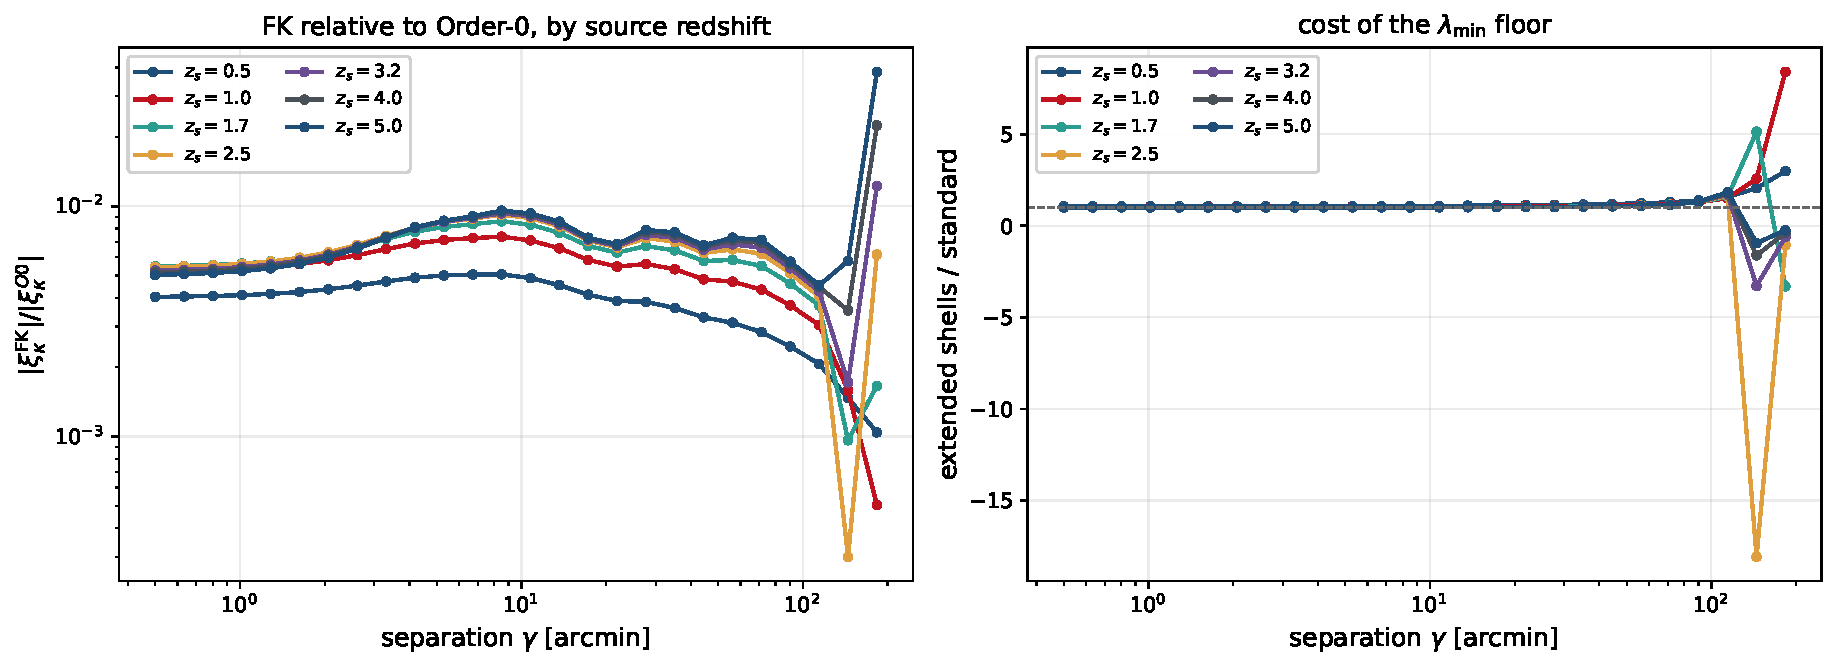
\includegraphics[width=\textwidth]{figures/redshift_lambdamin.pdf}
\caption{Left: the corrected FK contribution relative to Order-0 against
separation, at each source redshift. Right: the same FK calculation with
the tabulated shells extended from the deployed floor of $396.6$ Mpc down
to $50$ Mpc, divided by the standard one. The right panel is what the
$\lammin$ floor costs, and it is largest at low source redshift because the
kernel weight of the excised foreground grows as the source moves nearer.
Produced by \code{code/rebuild/fig\_redshift.py}.}
\label{fig:redshift}
\end{figure}
